\documentclass[10pt,fleqn]{article} % Default font size and left-justified equations
\usepackage[%
    pdftitle={Modélisation systèmes multiphysiques : Modélisation linéaire et non linéaire},
    pdfauthor={Xavier Pessoles}]{hyperref}
    
\input{style/new_style}
\input{style/macros_SII}
\usepackage{multicol}
\usepackage{standalone}
\standaloneconfig{mode=buildnew}
\usepackage{siunitx}
\usepackage{wrapfig}
\fichetrue

%\fichefalse

%\proftrue
%\proffalse

\tdtrue
%\tdfalse

\courstrue
\coursfalse

\def\discipline{Sciences \\Industrielles de \\ l'Ingénieur}
\def\xxtete{Sciences Industrielles de l'Ingénieur}

\def\classe{MP}
\def\xxnumpartie{01 à 03}
\def\xxpartie{Modéliser des SLCI et prédiction des performances}


\def\xxnumchapitre{Chapitre 1 \vspace{.2cm}}
\def\xxchapitre{\hspace{.12cm} Modélisation multiphysique}


\def\xxtitreexo{\noindent Escalier mécanique\\
Téléphérique Vanoise Express}
\def\xxsourceexo{\hspace{.2cm} \footnotesize{CCP MP 2014 \& E3A PSI 2014}}


\def\xxposongletx{2}
\def\xxposonglettext{1.45}
\def\xxposonglety{20}
%\def\xxonglet{Part. 1 -- Ch. 3}
\def\xxonglet{\textsf{Cy 01 à 03}}

\def\xxactivite{DS 2}
\def\xxauteur{\textsl{Xavier Pessoles}}

\def\xxcompetences{%
\textsl{%
\textbf{Savoirs et compétences :}\\
%Les sources sont associées par un \emph{hacheur série}. La détermination des grandeurs électriques associées à ce montage permet de conclure vis à vis du cahier des charges.
%\noindent \textbf{Résoudre :} à partir des modèles retenus :
%\begin{itemize}[label=\ding{112},font=\color{ocre}] 
%\item choisir une méthode de résolution analytique, graphique, numérique;
%\item mettre en \oe{}uvre une méthode de résolution.
%\end{itemize}
%\begin{itemize}[label=\ding{112},font=\color{ocre}] 
%\item \textit{Rés -- C1.1 :} Loi entrée sortie géométrique et cinématique -- Fermeture géométrique.
%\end{itemize}
%
%\noindent \textit{Mod2 -- C4.1 :} Représentation par schéma-blocs.
}}

\def\xxfigures{
%\includegraphics[width=.9\linewidth]{images/fig_01}
}%figues de la page de garde


\def\xxpied{%
Cycle 01 et 02\\
\xxactivite%
}

\setcounter{secnumdepth}{5}
%---------------------------------------------------------------------------

\usepackage{pgfplots}
\begin{document}
%\defimages{images}
%\chapterimage{png/Fond_Cin}
\input{style/new_pagegarde}
\vspace{4cm}
\pagestyle{fancy}
\thispagestyle{plain}
\def\pathfig{images2}
\def\columnseprulecolor{\color{ocre}}
\setlength{\columnseprule}{0.4pt} 

%\defimages2{images}

%\begin{multicols}{2}
%%%%%%%%%%%%%%%%%%%%%%%%%%%%%%%%%%%%%
\section{Escalier mécanique}
\subsection{Présentation}
\noindent\begin{minipage}[c]{.6\linewidth}
Un escalier mécanique, appelé aussi escalier roulant ou Escalator (nom déposé par la société Otis), est un élévateur adapté au transport de personnes. Sa fonction principale est de faciliter le déplacement des piétons entre deux points de différentes hauteurs. 

Depuis son invention en 1892 (à New York) par l’américain Jesse W. Reno, le système n’a pas cessé d’évoluer pour s’adapter aux nouvelles contraintes économiques, environnementales et sécuritaires.

\end{minipage}\hfill
\begin{minipage}[c]{.36\linewidth}
\begin{center}
\includegraphics[width=.95\linewidth]{images/fig_00}
\end{center}
\end{minipage}

\begin{center}
\includegraphics[width=.95\linewidth]{images/fig_00_bis}
\end{center}

Le système doit répondre aux exigences suivantes 


\begin{center}
\includegraphics[width=.95\linewidth]{images/fig_00_ter}
\end{center}

%\newpage

%\subsection{Réglage des paramètres de l'asservissement}

\begin{obj}
La maîtrise de la vitesse permet d’économiser de l’énergie mais cela ne doit pas se faire au détriment du confort et de la sécurité. L’objectif de cette partie est d’identifier les paramètres et de régler l’asservissement en vitesse afin d’avoir un comportement conforme au cahier des charges.
\end{obj}

La commande vectorielle du moteur asynchrone peut être modélisée autour du point de fonctionnement par l’asservissement en vitesse illustré par le schéma-blocs suivant. 
\begin{center}
	\includegraphics[width=\linewidth]{images/fig_01}
\end{center}

\begin{center}
	\includegraphics[width=\linewidth]{images/fig_02}
\end{center}

\subsection{Identification des caractéristiques : $c_f (t)$, $J$ et $f_v$}

On prendra $C(p) = 1$.

\subparagraph{}
\textit{Exprimer la vitesse du rotor $\Omega_m (p)$ en fonction de la consigne $\Omega_c (p)$ et du couple de frottement $C_f (p)$.}

\subparagraph{}
\textit{Donner l’expression de la constante de temps $\tau $du système en fonction de $J$, $K_a$ , et $f_v$.}
	
\subparagraph{}
\textit{Déterminer $\omega_{\infty}=\lim\limits_{t\to \infty} \omega_m (t)$ pour un échelon de consigne $\omega_c (t)=\omega_{c0}$ et un couple résistant supposé constant : $c_f (t)= C_{f0}$.}

\subparagraph{}
\textit{À partir des trois essais à vide donnés sur la figure suivante, tracer les graphes $\omega_{\infty}=g_1 (\omega_{c0})$ et $\tau=g_2 (\omega_{c0}$). Proposer un modèle d’identification pour les fonctions $g_1$ et $g_2$ . En déduire les valeurs de $C_{f0}$, $f_v$ et $J$.} 

\begin{center}
	\includegraphics[width=\linewidth]{images/fig_03}
\end{center}


On prendra $J=\SI{0,08}{kg.m^2}$ et $f_v=\SI{0}{N.m.s}$ pour la suite du sujet.


\subsection{Réglage du correcteur Proportionnel Intégral (PI)}
On choisit d’utiliser un correcteur Proportionnel Intégral modélisable par la fonction de transfert :
$C(p)=K\dfrac{1+p}{p}$  avec $K\in \mathbb{R}^+$.



\subparagraph{}
\textit{Justifier, vis-à-vis du cahier des charges, l’utilisation d’un correcteur Proportionnel Intégral.}



\subparagraph{}
\textit{Une simulation pour différentes valeurs du gain $K$ est représentée sur les figures suivantes. Compléter le tableau du document réponse à l’aide des différentes courbes. Donner la valeur de $K$ permettant de valider l’ensemble des critères: «~rapidité~», «~amortissement», «~précision~», «~facteur de confort~».}

\begin{center}
	\includegraphics[width=.8\linewidth]{images/fig_04}
	
	\includegraphics[width=.8\linewidth]{images/fig_05}
	
	\includegraphics[width=.8\linewidth]{images/fig_06}
\end{center}

\subparagraph{}
\textit{Donner l’expression de la fonction de transfert en boucle ouverte : $H_{\text{BO}} (p) =\dfrac{\Omega_m (p)}{\varepsilon (p)}$.}


\subparagraph{}
\textit{Tracer sur le document réponse la réponse fréquentielle dans le plan de Bode de $H_{\text{BO}}(p)$ (diagrammes asymptotiques + courbes réelles) pour la valeur de $K $ déterminée à la question 6. Faire apparaître, la marge de phase de l’asservissement puis conclure sur la capacité de l’asservissement à respecter le critère de stabilité du cahier des charges.}




\section{Étude du téléphérique Vanoise Express}
\subsection{Présentation}

\noindent\begin{minipage}[c]{.6\linewidth}

Noël 2003, le téléphérique Vanoise Express relie enfin les domaines skiables de La Plagne et Les Arcs, donnant naissance à paradiski, un domaine skiable de 425 km, le troisième plus grand de France.

	Le Vanoise Express est une prouesse technologique de 16.5 millions €. C’est le plus grand téléphérique de ce type jamais construit au monde. Il est réalisé par la société POMAGALSKI. C’est un téléphérique sans pylônes, d’une seule portée de gare à gare, ce qui permet de diminuer l’impact sur l’environnement et de préserver la beauté du paysage. L’utilisation de cabines à deux étages permet de réduire le volume des cabines et des gares, améliorant l’esthétique de l’ensemble.
	
	La solution retenue est constituée de deux lignes parallèles portant chacune une seule cabine. Contrairement à la plupart des téléphériques, les deux lignes sont entièrement indépendantes, ce qui signifie qu’une cabine n’est pas le contrepoids de l’autre. Ainsi, en cas de problème sur une cabine, la liaison entre les deux stations n’est pas interrompue.


\end{minipage}\hfill
\begin{minipage}[c]{.36\linewidth}
\begin{center}
\includegraphics[width=.95\linewidth]{images2/fig_00}
\end{center}
\end{minipage}

\vspace{.25cm}
Dans ce qui suit, on désire respecter les critères suivants du cahier des charges partiel :
\begin{center}
	\includegraphics[width=\linewidth]{images2/fig_01}
\end{center}

En effet, afin de respecter les consignes de vitesse pour un trajet entre «~Les Arcs~» et «~La Plagne~», il est nécessaire que l’asservissement de vitesse des moteurs à courant continu ait des qualités en précision, stabilité et rapidité.


\subsection{Modélisation du moteur à courant continu}
\begin{multicols}{2}

Hypothèses et données :
\begin{itemize}
\item on suppose les conditions initiales nulles;
\item les deux moteurs sont et fonctionnent de manière parfaitement identique;
\item $L=\SI{0,59}{mH}$ inductance d’un moteur;
\item $R=\SI{0,0386}{\Omega}$ résistance interne d’un moteur;
\item $f=\SI{6}{N.m.s/rad}$ coefficient de frottement visqueux équivalent ramené sur l’axe des moteurs;
\item $J=\SI{800}{kg.m^2}$ moment d’inertie total des pièces en rotation, ramené sur l’axe des moteurs; 
\item $c_m(t)=k_Ti(t)$ avec $k_T=\SI{5.67}{Nm/A}$ (constante de couple d’un moteur);
\item $e(t)=k_E\omega_m(t)$ avec $k_T=\SI{5.77}{Vs/rad}$   (constante électrique d’un moteur)
\item équations de la dynamique : $2c_m(t)-c_r(t)=K\omega_m(t)+f\omega_m(t)$.
\end{itemize}

\vspace{1.7cm}

Notations :

\begin{itemize}
\item on notera $F(p)$ la transformée de Laplace d’une fonction du temps $f(t)$;
\item $u(t)$ tension d’alimentation des moteurs;
\item $i(t)$ intensité traversant un moteur;
\item $e(t)$ force contre électromotrice d’un moteur;
\item $\omega_m(t)$ vitesse de rotation d’un moteur;
\item $c_m(t)$ couple d’un seul moteur;
\item $c_r(t)$ couple de perturbation engendré par le poids du téléphérique dans une pente et par l’action du vent, ramené sur l’axe des moteurs.
\end{itemize}
\end{multicols}

\subparagraph{}
\textit{Le schéma-blocs de la double motorisation étant fourni ci-après, déterminez les fonctions de transfert $G_1(p)$, $G_2(p)$, $G_3(p)$ et $G_4(p)$ écrites dans le domaine de Laplace.}

\begin{center}
	\includegraphics[width=\linewidth]{images2/fig_02}
\end{center}

\subparagraph{}
\textit{$\Omega_m(p)$ peut se mettre sous la forme :  $\Omega_m(p)=F_1(p)U(p)-F_2(p)C_r(p)$. Exprimer les fonctions $F_1(p)$ et $F_1(p)$ en fonction de $G_1(p)$, $G_2(p)$, $G_3(p)$ et $G_4(p)$.}


On donne les résultats d’une simulation réalisée sur l’ensemble de la motorisation, constituée des deux moteurs à courant continu :
\begin{enumerate}
\item la première courbe représente la réponse en vitesse à un échelon de tension $u(t)$ d’amplitude \SI{100}{V} (le couple de perturbation $c_r(t)$ est nul);
\item la seconde courbe représente la réponse en vitesse à un échelon de couple de perturbation $c_r(t)$ d’amplitude \SI{1000}{N.m} (la tension $u(t)$ est nulle).
\end{enumerate}



\noindent\begin{minipage}[c]{.48\linewidth}
\begin{center}
\includegraphics[width=\linewidth]{images2/fig_06_a}

\textit{Réponse en vitesse à un échelon de tension $u(t)$ d’amplitude \SI{100}{V}.}
\end{center}

\end{minipage}\hfill
\begin{minipage}[c]{.48\linewidth}
\begin{center}
\includegraphics[width=\linewidth]{images2/fig_06_b}

\textit{Réponse en vitesse à un échelon de couple de perturbation $c_r(t)$ d’amplitude \SI{1000}{N.m}.}
\end{center}
\end{minipage}



\subparagraph{}
\textit{Choisissez et justifiez un modèle d’identification de ces fonctions (premier ordre, second ordre etc...). Déterminez numériquement les deux fonctions $F_1(p)$ et $F_2(p)$ par identification.}


En faisant l’approximation que les deux fonctions $F_1(p)$ et $F_2(p)$ ont sensiblement le même dénominateur, le schéma bloc ci-dessus peut se mettre sous la forme suivante :
\begin{center}
	\includegraphics[width=\linewidth]{images2/fig_03}
\end{center}


\subparagraph{}
\textit{Donnez la valeur numérique des trois constantes $B$, $D$ et $T$.}

La motorisation modélisée ci-dessus est insérée dans une boucle d’asservissement de vitesse.

\begin{center}
	\includegraphics[width=\linewidth]{images2/fig_04}
\end{center}

\begin{itemize}
\item La consigne de vitesse $v_c(t)$ est donnée en entrée. Elle est convertie en une tension $\rho_c(t)$ avec le gain $F$.
\item Une génératrice tachymétrique de gain $\mu=\SI{0.716}{V.s/rad}$ transforme la vitesse de rotation $\omega_m(t)$ du moteur en une tension $\rho_m(t)$.
\item Un correcteur de fonction de transfert $C(p)$ corrige la différence $\varepsilon(t)=\rho_c(t)- \rho_m(t)$ et l’envoie à un amplificateur de gain $A$, qui alimente les deux moteurs électriques.
\item La vitesse de rotation des moteurs $\omega_m(t)$ est transformée en vitesse du téléphérique $v(t)$ avec le gain $E$.
\end{itemize}

\subparagraph{}
\textit{Déterminez l’expression du gain $E$. Faire une application numérique.}

\subparagraph{}
\textit{Déterminez l’expression du gain $F$ pour que $\varepsilon(t)=0$ entraîne $v_c(t)=v(t)$. Faire une application numérique.}

Par transformation du schéma bloc, le système est mis en retour unitaire. On obtient le résultat ci-dessous :
\begin{center}
	\includegraphics[width=\linewidth]{images2/fig_05}
\end{center}

	Les coefficients $E$ et $F$ calculés précédemment sont intégrés dans les nouveaux coefficients $A’$ et $G$. Pour la suite, on continuera avec les valeurs suivantes : $A'\cdot B=3\cdot 10^{-4}\;\text{sN}$; $G=6\cdot 10^{-5}\;\text{m/(sNm)}$ et $T=\SI{0,47}{s}$.
	
	
On se propose de tester successivement 3 correcteurs, et de retenir celui qui permet de respecter le cahier des charges.

\subsection{Utilisation d'un correcteur proportionnel}
$C(p)=C_0=1$.


\subparagraph{}
\textit{Justifiez en quelques mots que le système est stable avec ce correcteur.}

\subparagraph{}
\textit{On suppose $C_r(p)=0$. Calculez en fonction de $C_0$, $A’$, $B$, $G$ et $V_0$ l’expression de l’écart statique en suivi de consigne $\varepsilon'_s$ engendré par une consigne en échelon d’amplitude $V_0=\SI{12}{m/s}$. Faire l’application numérique.}

\vspace{.5cm}

On suppose $V_c(p)=0$.
\subparagraph{}
\textit{Calculez en fonction de $C_0$, $A’$, $B$, $G$ et $C_{r0}$ l’expression de l’écart statique en régulation $\varepsilon''_s$ engendré par une perturbation en échelon d’amplitude $C_{r0}=\SI{-7270}{Nm}$ qui modéliserait la descente des Arcs. Faire l’application numérique.}

\subparagraph{}
\textit{Faire également une application numérique si $C_{r0}=\SI{7460}{Nm}$ qui modéliserait la montée vers La Plagne.}

\subparagraph{}
\textit{Donnez numériquement l’écart statique total $\varepsilon_s=\varepsilon'_s+ \varepsilon''_s$  dans les deux cas suivants : descente des Arcs et montée vers La Plagne.}

\subparagraph{}
\textit{Existe-t-il une valeur réaliste de $C_0$ pour laquelle le critère «~Écart statique en vitesse en présence d’une perturbation échelon~» serait vérifié ? Justifiez.}


\subsection{Utilisation d'un correcteur intégral}

On choisit maintenant le correcteur $C(p)=\dfrac{C_i}{p}$.

\subparagraph{}
\textit{Donnez l’expression de la fonction de transfert en boucle ouverte du système, notée $\text{FTBO}(p)$. Faire l’application numérique pour $C_i=1$.}

\subparagraph{}
\textit{Tracez le diagramme asymptotique de Bode de $\text{FTBO}(p)$. Tracez également l’allure des courbes.}

\subparagraph{}
\textit{Quelles valeurs numériques de $C_i$ permettent de respecter le critère de «~Marge de phase~» du cahier des charges ?}

\subparagraph{}
\textit{Ces valeurs numériques de $C_i$ permettent-elles de respecter le critère de «~Pulsation de coupure en boucle ouverte~» du cahier des charges ? Justifiez.}

\subparagraph{}
\textit{On suppose Cr(p)=0. Calculez numériquement l’écart statique en suivi de consigne $\varepsilon'_s$ engendré par une consigne en échelon d’amplitude $V_0=\SI{12}{m/s}$.}

\subparagraph{}
\textit{On suppose $V_c(p)=0$. Calculez numériquement l’écart statique en régulation $\varepsilon''_s$ engendré par une perturbation échelon d’amplitude $C_{r0}=\SI{-7270}{N.m}$ qui modéliserait la descente des «~Arcs~».}

\subparagraph{}
\textit{Donnez numériquement l’écart statique total $\varepsilon_s=\varepsilon'_s+ \varepsilon''s$. Le critère «~Écart statique en vitesse en présence d’une perturbations échelon~» est-il vérifié ? Justifiez.}

\vspace{.5cm}

On suppose $C_r(p)=0$.
\subparagraph{}
\textit{Calculez l’expression de l’écart de traînage $\varepsilon_v$ engendré par une consigne en rampe unitaire. Existe-t-il une valeur de   réaliste qui permette de vérifier le critère «~Écart de traînage (ou écart dynamique) en vitesse en l’absence de perturbations~» ? Justifiez.}

\subsection{Utilisation d’un double correcteur intégral et d’un correcteur à avance de phase}


On décide d’utiliser le correcteur $C(p)=C_a(p)\dfrac{1}{p^2}$, produit de la fonction $C_a(p)=K\dfrac{1+a\tau p}{1+\tau p}$  avec $a>1$ (correcteur dont la fonction est d’ajouter de la phase) et d’un double intégrateur.
	On donne en fin de document réponse le diagramme de Bode de la fonction $H(p)=\dfrac{A'BG}{p^2\left(1+T p\right)}$, qui est la fonction de transfert en boucle ouverte du système sans $C_a(p)$   (c’est-à-dire pour $C_a(p)=1$).



\subparagraph{}
\textit{Montrez que le système n’est pas stable sans la fonction  $C_a(p)$ ?}

	La fonction $C_a(p)$ va nous permettre de stabiliser le système et de respecter les critères de «~Marge de phase~» et de «~Pulsation de coupure en boucle ouverte~». Pour cela, il faut suivre la démarche suivante.

\subparagraph{}
\textit{Combien de degrés de phase faut-il ajouter à la pulsation \SI{1}{rad/s} pour obtenir une phase de $-135\degres$ ?}

\subparagraph{}
\textit{Tracez en fonction de $a$, $\tau$ et $K$ les diagrammes asymptotiques de Bode (amplitude et phase) du correcteur $C_a(p)=K\dfrac{1+a\tau p}{1+\tau p}$  avec a>1. Précisez clairement les amplitudes ou les phases de toutes les asymptotes horizontales en fonction des différents paramètres. Précisez de même les pulsations des points particuliers.}

\subparagraph{}
\textit{La phase maximum $\varphi_{\text{max}}$ ajoutée par $C_a(p)$ peut être calculée par la formule : $\sin \varphi_{\text{max}}=\dfrac{a-1}{a+1}$ . Calculez numériquement $a$ pour obtenir la remontée de phase déterminée sur le diagramme de Bode à la question 30.}

Pour cette question, on pourra utiliser les propriétés de symétrie de la courbe de phase. 

\subparagraph{}
\textit{Donnez l’expression en fonction de $a$ et $\tau$ de la pulsation $\omega$ pour laquelle la courbe de phase atteint son maximum.}

\subparagraph{}
\textit{En déduire la valeur numérique de $\tau$ pour que $\varphi_{\text{max}}$ soit ajoutée à la pulsation \SI{1}{rad/s}.}

\subparagraph{}
\textit{Calculez numériquement la valeur à donner à $K$ pour respecter les critères de «~Marge de phase~» et de «~Pulsation de coupure en boucle ouverte~» du cahier des charges ? Précisez la démarche utilisée.}

\subparagraph{}
\textit{Les critères «~Écart statique en vitesse en présence d’une perturbation échelon~» et  «~Écart de traînage (ou écart dynamique) en vitesse en l’absence de perturbations~» sont-ils vérifiés ? Justifiez.}

\subparagraph{}
\textit{Ce correcteur permet-il de vérifier les critères du cahier des charges ? Justifiez.}

\end{document}

\begin{center}
	\includegraphics[width=\linewidth]{images/fig_02}
\end{center}

\begin{center}
	\includegraphics[width=\linewidth]{images/fig_02}
%\textit{Diagramme de Bode (gain uniquement) du système corrigé.}
\end{center}

\subparagraph{}
\textit{}
\ifprof
\begin{corrige}
\end{corrige}
\else
\fi
